\documentclass{beamer}

\usepackage{graphicx}
\usepackage{textpos}
\usepackage{listings}
\usepackage{lstautogobble}

\usetheme{Madrid}
\useoutertheme{miniframes} % Alternatively: miniframes, infolines, split

% Setup the university's color pallette
\definecolor{UIUCorange}{RGB}{19, 41, 75} % UBC Blue (primary)
\definecolor{UIUCblue}{RGB}{232, 74, 39} % UBC Grey (secondary)

\definecolor{codegreen}{rgb}{0,0.6,0}
\definecolor{codegray}{rgb}{0.5,0.5,0.5}
\definecolor{codepurple}{rgb}{0.58,0,0.82}
\definecolor{backcolour}{rgb}{0.95,0.95,0.92}

\lstdefinestyle{python}{
  backgroundcolor=\color{backcolour},   
  commentstyle=\color{codegreen},
  keywordstyle=\color{magenta},
  numberstyle=\tiny\color{codegray},
  stringstyle=\color{codepurple},
  basicstyle=\ttfamily\footnotesize,
  breakatwhitespace=false,         
  belowskip=-0.5em,
  breaklines=true,                 
  captionpos=b,                    
  keepspaces=true,                 
  numbers=left,                    
  numbersep=5pt,                  
  showspaces=false,                
  showstringspaces=false,
  showtabs=false,                  
  tabsize=2
}

\lstset{style=python}

\AtBeginSection[]{
    \begin{frame}
        \vfill
        \centering
        \begin{beamercolorbox}[sep=8pt,center,shadow=true,rounded=true]{title}
            \usebeamerfont{title}\insertsectionhead\par%
        \end{beamercolorbox}
        \vfill
    \end{frame}
}
% Setup the university's color pallette
\definecolor{UIUCorange}{RGB}{19, 41, 75} % UBC Blue (primary)
\definecolor{UIUCblue}{RGB}{232, 74, 39} % UBC Grey (secondary)


\setbeamercolor{palette primary}{bg=UIUCorange,fg=white}
\setbeamercolor{palette secondary}{bg=UIUCblue,fg=white}
\setbeamercolor{palette tertiary}{bg=UIUCblue,fg=white}
\setbeamercolor{palette quaternary}{bg=UIUCblue,fg=white}
\setbeamercolor{structure}{fg=UIUCorange} % itemize, enumerate, etc
\setbeamercolor{section in toc}{fg=UIUCblue} % TOC sections

\setbeamercolor{subsection in head/foot}{bg=UIUCorange,fg=UIUCblue}
\setbeamercolor{subsection in head/foot}{bg=UIUCorange,fg=UIUCblue}

\usepackage[utf8]{inputenc}
\usepackage{graphicx}

%Information to be included in the title page:
\title{\textbf{Lists}}
\author{\textbf{David H Smith IV}}
\institute[\textbf{UIUC}]{\textbf{University of Illinois Urbana-Champaign}}
\date{\textbf{Tues, Thu 21 2021}}

\setbeamertemplate{title page}[default][colsep=-4bp,rounded=true]
\addtobeamertemplate{title page}{\vspace{3\baselineskip}}{}
\addtobeamertemplate{title page}{
  \begin{textblock*}{\paperwidth}(-1.0em, -1.2em)
    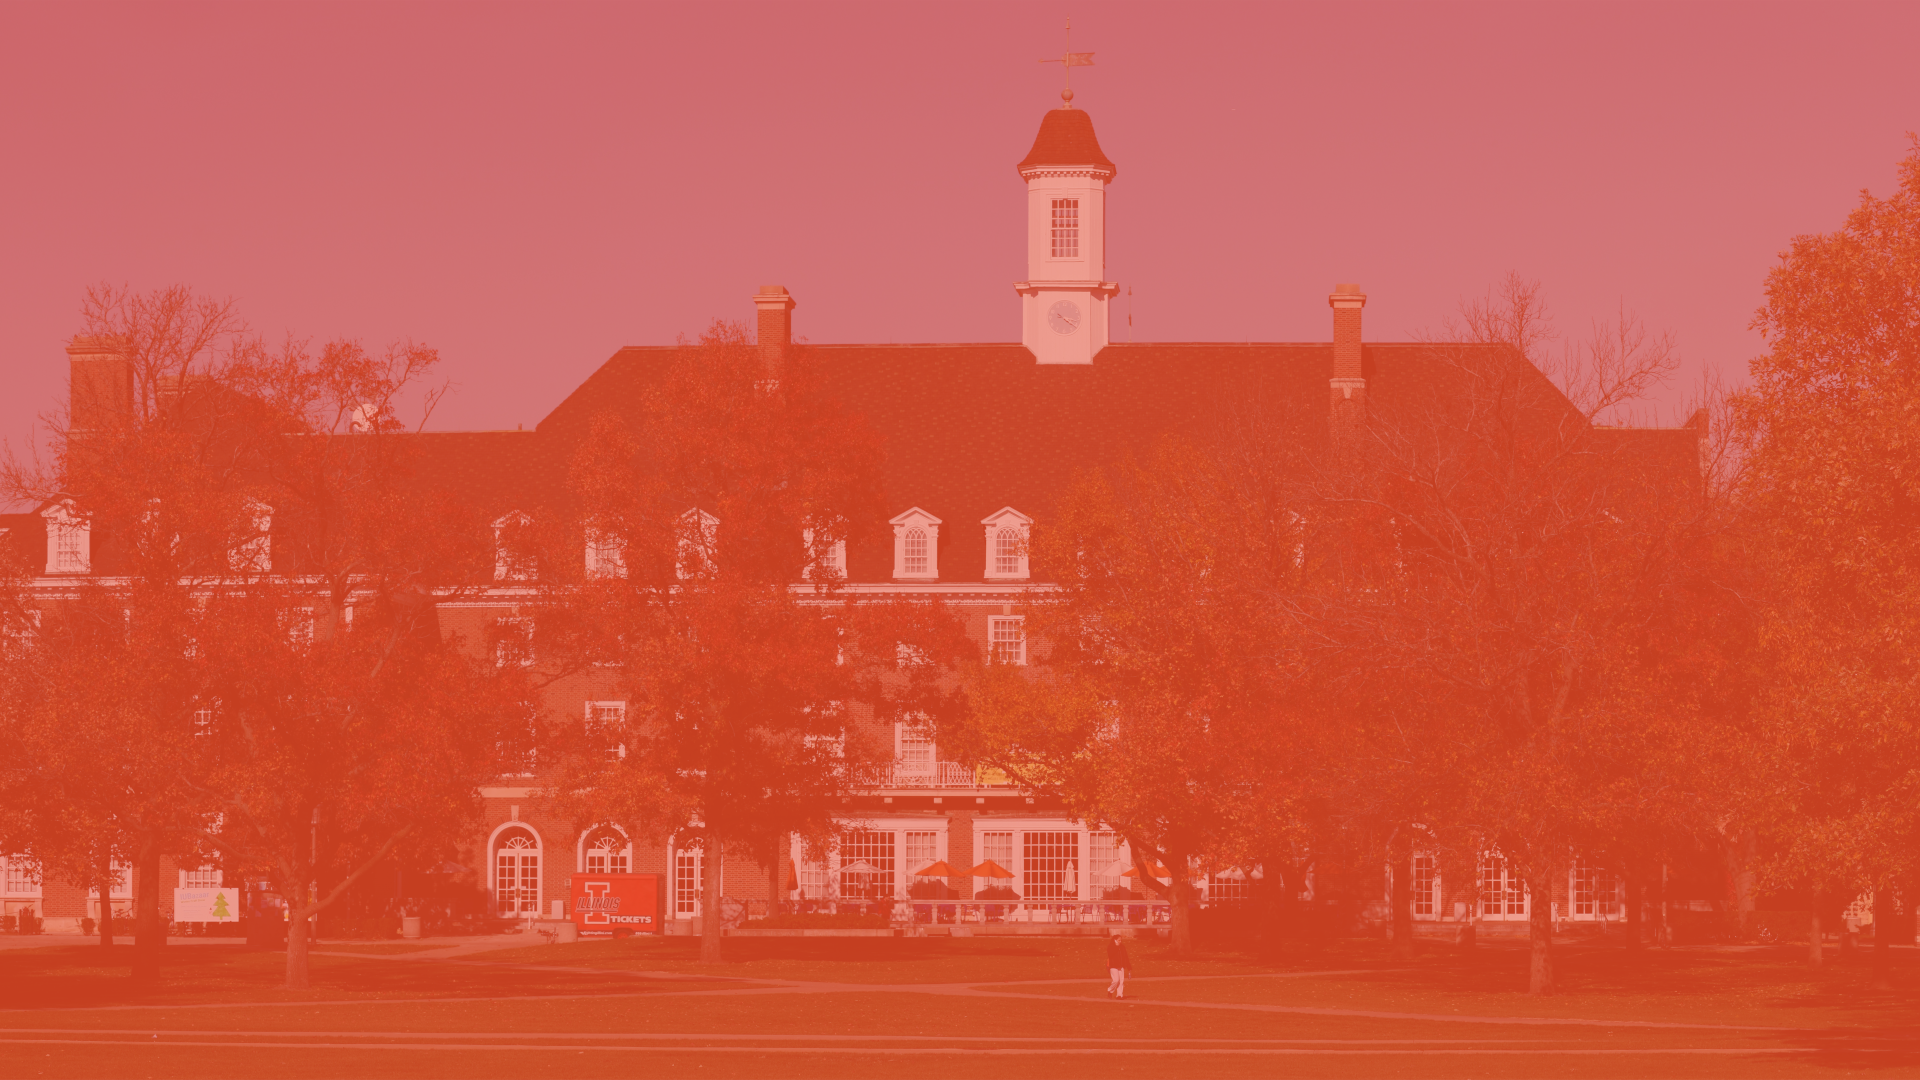
\includegraphics[width=\paperwidth, height=\paperheight]{imgs/uiuc.png}
  \end{textblock*} 
}{}

\begin{document}

\frame{\titlepage}

\section{Reminders}

%
% Slide 1
%
\begin{frame}
  \frametitle{Reminders}
  \begin{itemize}
    \item 
  \end{itemize}
\end{frame}

\section{Lists}

%
% Slide 2
%
\begin{frame}[fragile]
  \frametitle{Poll Question: Tracing}
  What is the value of \lstinline|x|.
  \begin{lstlisting}[language=Python, autogobble]
  x = [v+v for v in ['1', '2', '3']]
  \end{lstlisting}
  \vfill
  \begin{enumerate}[A]
    \item \lstinline|['11', '22', '33']| 
    \item \lstinline|['1', '2', '3']|
    \item \lstinline|[1, 4, 9]|
    \item TypeError
  \end{enumerate}
\end{frame}

%
% Slide 2
%
\begin{frame}[fragile]
  \frametitle{List Comprehensions}
  \begin{lstlisting}[language=Python, autogobble]
  # Basic list comprehension
  [expression for value in sequence]

  # Conditional list comprehension with if
  [expresssion for value in sequence if condition]

  #Conditional list comprehension with if-else
  [expresssion if conditition else <default> for value in sequence]
  \end{lstlisting}
  \vfill
  \begin{itemize}
    \item Doesn't enable any new functionality 
    \item \textit{Syntactic Sugar: } Makes code more efficient to write
  \end{itemize}
\end{frame}

%
% Slide 2
%
\begin{frame}[fragile]
  \frametitle{Poll Question: List Comprehension}
  What is the value of \lstinline|y|.
  \begin{lstlisting}[language=Python, autogobble]
  y = [c for c in 'alma mater' if c in 'aeiou']
  \end{lstlisting}
  \vfill
  \begin{enumerate}[A]
    \item \lstinline|'alma mater'|
    \item \lstinline|['alma mater']|
    \item \lstinline|'aaae'|
    \item \lstinline|['a', 'a', 'a', 'e']|
  \end{enumerate}
\end{frame}

\end{document}
